%%%%%%%%%%%%%%%%%%%%%%%%%%%%%%%%%%%%%%%%%%%%%%%%%%%%%%%%%%%%%%%%%%%%
% Authors: A. Herrera-Poyatos, F. Herrera
% Tittle: Algoritmo memético equilibrado con diversificación voraz
% 							 CAEPIA 2015
%%%%%%%%%%%%%%%%%%%%%%%%%%%%%%%%%%%%%%%%%%%%%%%%%%%%%%%%%%%%%%%%%%%%

\section[AMEDV]{Algoritmo Memético Equilibrado con Diversificación Voraz}

	\subsection*{Funcionamiento}

		\begin{frame}{Algoritmo Memético Equilibrado con Diversificación Voraz}
			
			\fontsize{8}{10}\selectfont
			\begin{tikzpicture}[
			every node/.style={circle, inner sep=0pt, text width=1.85cm, align=center, node distance=2cm}]
			
			\node [fill=blue!10] (i) {Inicializar $P$};
			\node [fill=blue!20, right = of $(i)$] (s) {Selección Aleatoria Adyacente};
			\node [fill=blue!40, right = 5cm of $(s)$] (co) {Competición};
			\node [fill=blue!30, above = 0.25cm of {$(s)!0.5!(co)$}] (c) {Cruce};
			\node [fill=blue!50, below = 1cm of {$(s)!0.7!(co)$}] (dv) {Diversificación voraz};
			\node [fill=blue!60, below = 1cm of {$(s)!0.3!(co)$}] (bl) {Búsqueda local};
			
			\path[every node/.style={font=\sffamily\small}]
			(i) edge [->, >=stealth', line width=0.5mm] node {} (s)
			(s) edge [->, >=stealth', line width=0.5mm] node {} (c);

			\path[every node/.style={font=\sffamily\small}]
			(c) edge [->, >=stealth', line width=0.5mm] node {} (co);
			
			\path[every node/.style={font=\sffamily\small}]
			(co) edge [->, >=stealth', line width=0.5mm] node {} (dv);
			
			\path[every node/.style={font=\sffamily\small}]
			(dv) edge [->, >=stealth', line width=0.5mm] node {} (bl);

			\path[every node/.style={font=\sffamily\small}]
			(bl) edge [->, >=stealth', line width=0.5mm] node {} (s);
			
			\end{tikzpicture}
			
			
			\begin{tcolorbox}[colback=blue!5,colframe=blue!30]
				\centering
				\fontsize{10}{10}\selectfont
				\textbf{Algoritmo genético equilibrado con diversificación voraz \\ + \\ Búsqueda local}	
			\end{tcolorbox}
						
		\end{frame}
	
	\subsection*{Diversidad}

		\begin{frame}{Diversidad en la población de AMEDV}
			
			% Font size
			\fontsize{9}{10}\selectfont
			
			\centering 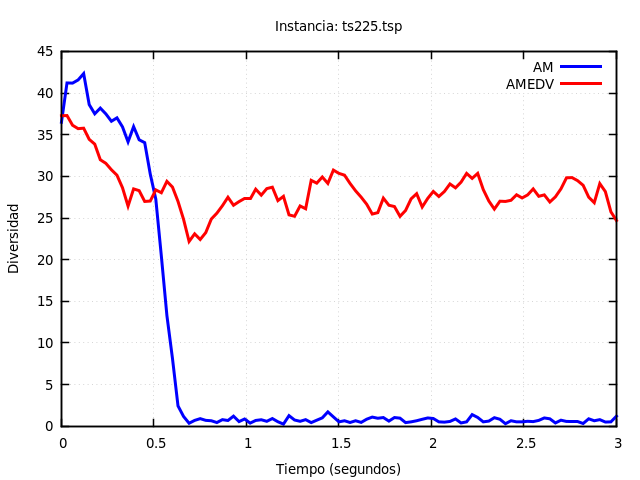
\includegraphics[width=7cm]{./Images/Diversity/AMEDV/png/ts225.png}
							
			\kern 4mm
			\fontsize{9}{10}\selectfont
			
			\begin{tcolorbox}[colback=blue!5,colframe=blue!30]
				\centering
				\textbf{La diversidad se controla mediante la diversificación voraz.}
			\end{tcolorbox}
			
		\end{frame}